% Options for packages loaded elsewhere
% Options for packages loaded elsewhere
\PassOptionsToPackage{unicode}{hyperref}
\PassOptionsToPackage{hyphens}{url}
\PassOptionsToPackage{dvipsnames,svgnames,x11names}{xcolor}
%
\documentclass[
  10pt,
  titlepage=false]{exam}
\usepackage{xcolor}
\usepackage{amsmath,amssymb}
\setcounter{secnumdepth}{-\maxdimen} % remove section numbering
\usepackage{iftex}
\ifPDFTeX
  \usepackage[T1]{fontenc}
  \usepackage[utf8]{inputenc}
  \usepackage{textcomp} % provide euro and other symbols
\else % if luatex or xetex
  \usepackage{unicode-math} % this also loads fontspec
  \defaultfontfeatures{Scale=MatchLowercase}
  \defaultfontfeatures[\rmfamily]{Ligatures=TeX,Scale=1}
\fi
\usepackage{lmodern}
\ifPDFTeX\else
  % xetex/luatex font selection
\fi
% Use upquote if available, for straight quotes in verbatim environments
\IfFileExists{upquote.sty}{\usepackage{upquote}}{}
\IfFileExists{microtype.sty}{% use microtype if available
  \usepackage[]{microtype}
  \UseMicrotypeSet[protrusion]{basicmath} % disable protrusion for tt fonts
}{}
\makeatletter
\@ifundefined{KOMAClassName}{% if non-KOMA class
  \IfFileExists{parskip.sty}{%
    \usepackage{parskip}
  }{% else
    \setlength{\parindent}{0pt}
    \setlength{\parskip}{6pt plus 2pt minus 1pt}}
}{% if KOMA class
  \KOMAoptions{parskip=half}}
\makeatother
% Make \paragraph and \subparagraph free-standing
\makeatletter
\ifx\paragraph\undefined\else
  \let\oldparagraph\paragraph
  \renewcommand{\paragraph}{
    \@ifstar
      \xxxParagraphStar
      \xxxParagraphNoStar
  }
  \newcommand{\xxxParagraphStar}[1]{\oldparagraph*{#1}\mbox{}}
  \newcommand{\xxxParagraphNoStar}[1]{\oldparagraph{#1}\mbox{}}
\fi
\ifx\subparagraph\undefined\else
  \let\oldsubparagraph\subparagraph
  \renewcommand{\subparagraph}{
    \@ifstar
      \xxxSubParagraphStar
      \xxxSubParagraphNoStar
  }
  \newcommand{\xxxSubParagraphStar}[1]{\oldsubparagraph*{#1}\mbox{}}
  \newcommand{\xxxSubParagraphNoStar}[1]{\oldsubparagraph{#1}\mbox{}}
\fi
\makeatother

\usepackage{color}
\usepackage{fancyvrb}
\newcommand{\VerbBar}{|}
\newcommand{\VERB}{\Verb[commandchars=\\\{\}]}
\DefineVerbatimEnvironment{Highlighting}{Verbatim}{commandchars=\\\{\}}
% Add ',fontsize=\small' for more characters per line
\usepackage{framed}
\definecolor{shadecolor}{RGB}{241,243,245}
\newenvironment{Shaded}{\begin{snugshade}}{\end{snugshade}}
\newcommand{\AlertTok}[1]{\textcolor[rgb]{0.68,0.00,0.00}{#1}}
\newcommand{\AnnotationTok}[1]{\textcolor[rgb]{0.37,0.37,0.37}{#1}}
\newcommand{\AttributeTok}[1]{\textcolor[rgb]{0.40,0.45,0.13}{#1}}
\newcommand{\BaseNTok}[1]{\textcolor[rgb]{0.68,0.00,0.00}{#1}}
\newcommand{\BuiltInTok}[1]{\textcolor[rgb]{0.00,0.23,0.31}{#1}}
\newcommand{\CharTok}[1]{\textcolor[rgb]{0.13,0.47,0.30}{#1}}
\newcommand{\CommentTok}[1]{\textcolor[rgb]{0.37,0.37,0.37}{#1}}
\newcommand{\CommentVarTok}[1]{\textcolor[rgb]{0.37,0.37,0.37}{\textit{#1}}}
\newcommand{\ConstantTok}[1]{\textcolor[rgb]{0.56,0.35,0.01}{#1}}
\newcommand{\ControlFlowTok}[1]{\textcolor[rgb]{0.00,0.23,0.31}{\textbf{#1}}}
\newcommand{\DataTypeTok}[1]{\textcolor[rgb]{0.68,0.00,0.00}{#1}}
\newcommand{\DecValTok}[1]{\textcolor[rgb]{0.68,0.00,0.00}{#1}}
\newcommand{\DocumentationTok}[1]{\textcolor[rgb]{0.37,0.37,0.37}{\textit{#1}}}
\newcommand{\ErrorTok}[1]{\textcolor[rgb]{0.68,0.00,0.00}{#1}}
\newcommand{\ExtensionTok}[1]{\textcolor[rgb]{0.00,0.23,0.31}{#1}}
\newcommand{\FloatTok}[1]{\textcolor[rgb]{0.68,0.00,0.00}{#1}}
\newcommand{\FunctionTok}[1]{\textcolor[rgb]{0.28,0.35,0.67}{#1}}
\newcommand{\ImportTok}[1]{\textcolor[rgb]{0.00,0.46,0.62}{#1}}
\newcommand{\InformationTok}[1]{\textcolor[rgb]{0.37,0.37,0.37}{#1}}
\newcommand{\KeywordTok}[1]{\textcolor[rgb]{0.00,0.23,0.31}{\textbf{#1}}}
\newcommand{\NormalTok}[1]{\textcolor[rgb]{0.00,0.23,0.31}{#1}}
\newcommand{\OperatorTok}[1]{\textcolor[rgb]{0.37,0.37,0.37}{#1}}
\newcommand{\OtherTok}[1]{\textcolor[rgb]{0.00,0.23,0.31}{#1}}
\newcommand{\PreprocessorTok}[1]{\textcolor[rgb]{0.68,0.00,0.00}{#1}}
\newcommand{\RegionMarkerTok}[1]{\textcolor[rgb]{0.00,0.23,0.31}{#1}}
\newcommand{\SpecialCharTok}[1]{\textcolor[rgb]{0.37,0.37,0.37}{#1}}
\newcommand{\SpecialStringTok}[1]{\textcolor[rgb]{0.13,0.47,0.30}{#1}}
\newcommand{\StringTok}[1]{\textcolor[rgb]{0.13,0.47,0.30}{#1}}
\newcommand{\VariableTok}[1]{\textcolor[rgb]{0.07,0.07,0.07}{#1}}
\newcommand{\VerbatimStringTok}[1]{\textcolor[rgb]{0.13,0.47,0.30}{#1}}
\newcommand{\WarningTok}[1]{\textcolor[rgb]{0.37,0.37,0.37}{\textit{#1}}}

\usepackage{longtable,booktabs,array}
\usepackage{calc} % for calculating minipage widths
% Correct order of tables after \paragraph or \subparagraph
\usepackage{etoolbox}
\makeatletter
\patchcmd\longtable{\par}{\if@noskipsec\mbox{}\fi\par}{}{}
\makeatother
% Allow footnotes in longtable head/foot
\IfFileExists{footnotehyper.sty}{\usepackage{footnotehyper}}{\usepackage{footnote}}
\makesavenoteenv{longtable}
\usepackage{graphicx}
\makeatletter
\newsavebox\pandoc@box
\newcommand*\pandocbounded[1]{% scales image to fit in text height/width
  \sbox\pandoc@box{#1}%
  \Gscale@div\@tempa{\textheight}{\dimexpr\ht\pandoc@box+\dp\pandoc@box\relax}%
  \Gscale@div\@tempb{\linewidth}{\wd\pandoc@box}%
  \ifdim\@tempb\p@<\@tempa\p@\let\@tempa\@tempb\fi% select the smaller of both
  \ifdim\@tempa\p@<\p@\scalebox{\@tempa}{\usebox\pandoc@box}%
  \else\usebox{\pandoc@box}%
  \fi%
}
% Set default figure placement to htbp
\def\fps@figure{htbp}
\makeatother





\setlength{\emergencystretch}{3em} % prevent overfull lines

\providecommand{\tightlist}{%
  \setlength{\itemsep}{0pt}\setlength{\parskip}{0pt}}



 


\usepackage{ntheorem}
\RequirePackage{amsmath,amssymb,amsfonts,natbib}
\usepackage[a4paper,margin={.1\paperheight,.1\paperwidth},marginratio=1:1]{geometry}
\usepackage{enumerate}
\usepackage{epsfig}

\usepackage{csquotes}
\usepackage{fontspec}
\usepackage{polyglossia}

\setdefaultlanguage{french}
\setotherlanguage[variant=british]{english}

\usepackage{hyperref}
\usepackage{xcolor}

\newtheorem{definition}{Définition}
\newtheorem{notation}{Notation}
\newtheorem{lemma}{Lemme}
\newtheorem{proposition}{Proposition}
\newtheorem{corollary}{Corollaire}
\newtheorem{theorem}{Théorème}

% % % %
% Code SQL
% % % %



\usepackage{tikz}
\usetikzlibrary{shapes}


\providecommand{\og}{\guillemotleft}
\providecommand{\fg}{\guillemotright}

% % % %
% % % %
\rhead{\textsf{Licence 3 MIASHS-Math  \\2024--2025}}
\lhead{{\sf  MA15E045 BD5 Licence MIASHS \\ TD
%\notd
}}
% \rhead{\textsf{Master I ISIFAR  \\2023--2024}}
% \lhead{{\sf  BD Master I ISIFAR \\ TD
% %\notd
% }}
\cfoot{\thepage}





\renewcommand{\contentsname}{}
\lhead{{\sf  Base de données \\ CT 2024-01-08 12h-15h}}
\makeatletter
\@ifpackageloaded{tcolorbox}{}{\usepackage[skins,breakable]{tcolorbox}}
\@ifpackageloaded{fontawesome5}{}{\usepackage{fontawesome5}}
\definecolor{quarto-callout-color}{HTML}{909090}
\definecolor{quarto-callout-note-color}{HTML}{0758E5}
\definecolor{quarto-callout-important-color}{HTML}{CC1914}
\definecolor{quarto-callout-warning-color}{HTML}{EB9113}
\definecolor{quarto-callout-tip-color}{HTML}{00A047}
\definecolor{quarto-callout-caution-color}{HTML}{FC5300}
\definecolor{quarto-callout-color-frame}{HTML}{acacac}
\definecolor{quarto-callout-note-color-frame}{HTML}{4582ec}
\definecolor{quarto-callout-important-color-frame}{HTML}{d9534f}
\definecolor{quarto-callout-warning-color-frame}{HTML}{f0ad4e}
\definecolor{quarto-callout-tip-color-frame}{HTML}{02b875}
\definecolor{quarto-callout-caution-color-frame}{HTML}{fd7e14}
\makeatother
\makeatletter
\@ifpackageloaded{caption}{}{\usepackage{caption}}
\AtBeginDocument{%
\ifdefined\contentsname
  \renewcommand*\contentsname{Table of contents}
\else
  \newcommand\contentsname{Table of contents}
\fi
\ifdefined\listfigurename
  \renewcommand*\listfigurename{List of Figures}
\else
  \newcommand\listfigurename{List of Figures}
\fi
\ifdefined\listtablename
  \renewcommand*\listtablename{List of Tables}
\else
  \newcommand\listtablename{List of Tables}
\fi
\ifdefined\figurename
  \renewcommand*\figurename{Figure}
\else
  \newcommand\figurename{Figure}
\fi
\ifdefined\tablename
  \renewcommand*\tablename{Table}
\else
  \newcommand\tablename{Table}
\fi
}
\@ifpackageloaded{float}{}{\usepackage{float}}
\floatstyle{ruled}
\@ifundefined{c@chapter}{\newfloat{codelisting}{h}{lop}}{\newfloat{codelisting}{h}{lop}[chapter]}
\floatname{codelisting}{Listing}
\newcommand*\listoflistings{\listof{codelisting}{List of Listings}}
\makeatother
\makeatletter
\makeatother
\makeatletter
\@ifpackageloaded{caption}{}{\usepackage{caption}}
\@ifpackageloaded{subcaption}{}{\usepackage{subcaption}}
\makeatother
\makeatletter
\@ifpackageloaded{fontawesome5}{}{\usepackage{fontawesome5}}
\makeatother
\usepackage{bookmark}
\IfFileExists{xurl.sty}{\usepackage{xurl}}{} % add URL line breaks if available
\urlstyle{same}
\hypersetup{
  colorlinks=true,
  linkcolor={blue},
  filecolor={Maroon},
  citecolor={Blue},
  urlcolor={Blue},
  pdfcreator={LaTeX via pandoc}}


\author{}
\date{}
\begin{document}

\renewcommand{\contentsname}{}


\begin{figure}

\begin{minipage}{0.80\linewidth}

\begin{itemize}
\tightlist
\item
  \textbf{L3 MIASHS/Ingémath}
\item
  \textbf{\href{https://www.u-paris.fr}{Université Paris Cité}}
\item
  Année 2023-2024
\item
  \href{https://stephane-v-boucheron.fr/courses/bdd}{Course Homepage}\\
\item
  \href{https://moodle.u-paris.fr/course/view.php?id=2313}{Moodle}
\end{itemize}

\end{minipage}%
%
\begin{minipage}{0.20\linewidth}

\includegraphics[width=0.78125in,height=\textheight,keepaspectratio]{../images/UniversiteParis_monogramme_couleur_RVB.png}\end{minipage}%

\end{figure}%

\begin{tcolorbox}[enhanced jigsaw, leftrule=.75mm, colback=white, colframe=quarto-callout-warning-color-frame, opacityback=0, left=2mm, arc=.35mm, toprule=.15mm, breakable, rightrule=.15mm, bottomrule=.15mm]
\begin{minipage}[t]{5.5mm}
\textcolor{quarto-callout-warning-color}{\faExclamationTriangle}
\end{minipage}%
\begin{minipage}[t]{\textwidth - 5.5mm}

Les trois exercices (modélisation, normalisation, requêtes) portent sur
le schéma \texttt{nycflights} légèrement nettoyé.

\end{minipage}%
\end{tcolorbox}

\begin{figure}[H]

{\centering 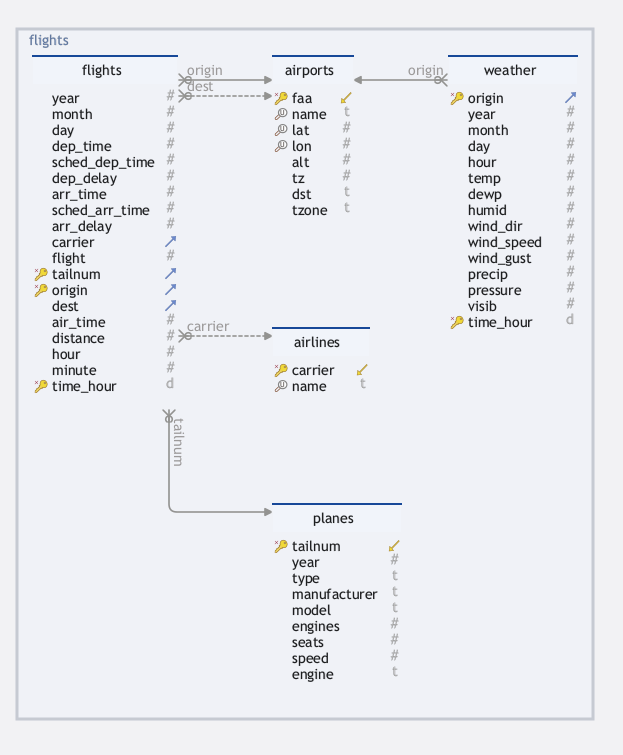
\includegraphics[width=0.8\linewidth,height=\textheight,keepaspectratio]{../images/nycflights_layout_crop.png}

}

\caption{NYCFlights en relationel à pattes de corbeau}

\end{figure}%

\newpage{}

\subsubsection{Définition du schéma en
SQL}\label{duxe9finition-du-schuxe9ma-en-sql}

\begin{figure}

\begin{minipage}{0.50\linewidth}

\begin{Shaded}
\begin{Highlighting}[]
\KeywordTok{CREATE} \KeywordTok{TABLE}\NormalTok{ airlines (}
\NormalTok{    carrier text }\KeywordTok{NOT} \KeywordTok{NULL}\NormalTok{,}
    \OtherTok{"name"}\NormalTok{ text }\KeywordTok{NULL}\NormalTok{,}
    \KeywordTok{CONSTRAINT}\NormalTok{ airlines\_pk }
        \KeywordTok{PRIMARY} \KeywordTok{KEY}\NormalTok{ (carrier),}
    \KeywordTok{CONSTRAINT}\NormalTok{ airlines\_un }
        \KeywordTok{UNIQUE}\NormalTok{ (name)}
\NormalTok{);}
\end{Highlighting}
\end{Shaded}

\begin{Shaded}
\begin{Highlighting}[]
\KeywordTok{CREATE} \KeywordTok{TABLE}\NormalTok{ airports (}
\NormalTok{    faa text }\KeywordTok{NOT} \KeywordTok{NULL}\NormalTok{,}
    \OtherTok{"name"}\NormalTok{ text }\KeywordTok{NULL}\NormalTok{,}
\NormalTok{    lat float8 }\KeywordTok{NULL}\NormalTok{,}
\NormalTok{    lon float8 }\KeywordTok{NULL}\NormalTok{,}
\NormalTok{    alt float8 }\KeywordTok{NULL}\NormalTok{,}
\NormalTok{    tz float8 }\KeywordTok{NULL}\NormalTok{,}
\NormalTok{    dst text }\KeywordTok{NULL}\NormalTok{,}
\NormalTok{    tzone text }\KeywordTok{NULL}\NormalTok{,}
    \KeywordTok{CONSTRAINT}\NormalTok{ airports\_pk }
        \KeywordTok{PRIMARY} \KeywordTok{KEY}\NormalTok{ (faa),}
    \KeywordTok{CONSTRAINT}\NormalTok{ airports\_un }
        \KeywordTok{UNIQUE}\NormalTok{ (name),}
    \KeywordTok{CONSTRAINT}\NormalTok{ airports\_un\_ll }
        \KeywordTok{UNIQUE}\NormalTok{ (lat, lon)}
\NormalTok{);}
\end{Highlighting}
\end{Shaded}

\end{minipage}%
%
\begin{minipage}{0.50\linewidth}

\begin{Shaded}
\begin{Highlighting}[]
\KeywordTok{CREATE} \KeywordTok{TABLE}\NormalTok{ weather (}
\NormalTok{    origin text }\KeywordTok{NOT} \KeywordTok{NULL}\NormalTok{,}
    \OtherTok{"year"}\NormalTok{ int4 }\KeywordTok{NULL}\NormalTok{,}
    \OtherTok{"month"}\NormalTok{ int4 }\KeywordTok{NULL}\NormalTok{,}
    \OtherTok{"day"}\NormalTok{ int4 }\KeywordTok{NULL}\NormalTok{,}
    \OtherTok{"hour"}\NormalTok{ int4 }\KeywordTok{NULL}\NormalTok{,}
    \OtherTok{"temp"}\NormalTok{ float8 }\KeywordTok{NULL}\NormalTok{,}
\NormalTok{    dewp float8 }\KeywordTok{NULL}\NormalTok{,}
\NormalTok{    humid float8 }\KeywordTok{NULL}\NormalTok{,}
\NormalTok{    wind\_dir float8 }\KeywordTok{NULL}\NormalTok{,}
\NormalTok{    wind\_speed float8 }\KeywordTok{NULL}\NormalTok{,}
\NormalTok{    wind\_gust float8 }\KeywordTok{NULL}\NormalTok{,}
\NormalTok{    precip float8 }\KeywordTok{NULL}\NormalTok{,}
\NormalTok{    pressure float8 }\KeywordTok{NULL}\NormalTok{,}
\NormalTok{    visib float8 }\KeywordTok{NULL}\NormalTok{,}
\NormalTok{    time\_hour timestamptz }\KeywordTok{NOT} \KeywordTok{NULL}\NormalTok{,}
    \KeywordTok{CONSTRAINT}\NormalTok{ weather\_pk }
        \KeywordTok{PRIMARY} \KeywordTok{KEY}\NormalTok{ (origin, time\_hour)}
\NormalTok{);}
\end{Highlighting}
\end{Shaded}

\begin{Shaded}
\begin{Highlighting}[]
\KeywordTok{ALTER} \KeywordTok{TABLE}\NormalTok{ weather }\KeywordTok{ADD} 
    \KeywordTok{CONSTRAINT}\NormalTok{ weather\_fk }
    \KeywordTok{FOREIGN} \KeywordTok{KEY}\NormalTok{ (origin) }
    \KeywordTok{REFERENCES}\NormalTok{ airports(faa) }
    \KeywordTok{ON} \KeywordTok{DELETE} \KeywordTok{CASCADE} 
    \KeywordTok{ON} \KeywordTok{UPDATE} \KeywordTok{CASCADE}\NormalTok{;}
\end{Highlighting}
\end{Shaded}

\end{minipage}%

\end{figure}%

\begin{Shaded}
\begin{Highlighting}[]
\KeywordTok{CREATE} \KeywordTok{TABLE}\NormalTok{ planes (}
\NormalTok{    tailnum text }\KeywordTok{NOT} \KeywordTok{NULL}\NormalTok{,}
    \OtherTok{"year"}\NormalTok{ int4 }\KeywordTok{NULL}\NormalTok{,}
    \OtherTok{"type"}\NormalTok{ text }\KeywordTok{NULL}\NormalTok{,}
\NormalTok{    manufacturer text }\KeywordTok{NULL}\NormalTok{,}
\NormalTok{    model text }\KeywordTok{NULL}\NormalTok{,}
\NormalTok{    engines int4 }\KeywordTok{NULL}\NormalTok{,}
\NormalTok{    seats int4 }\KeywordTok{NULL}\NormalTok{,}
\NormalTok{    speed int4 }\KeywordTok{NULL}\NormalTok{,}
\NormalTok{    engine text }\KeywordTok{NULL}\NormalTok{,}
    \KeywordTok{CONSTRAINT}\NormalTok{ planes\_pk   }\KeywordTok{PRIMARY} \KeywordTok{KEY}\NormalTok{ (tailnum)}
\NormalTok{);}
\end{Highlighting}
\end{Shaded}

\begin{figure}

\begin{minipage}{0.50\linewidth}

\begin{Shaded}
\begin{Highlighting}[]
\KeywordTok{CREATE} \KeywordTok{TABLE}\NormalTok{ flights (}
    \OtherTok{"year"}\NormalTok{ int4 }\KeywordTok{NULL}\NormalTok{,}
    \OtherTok{"month"}\NormalTok{ int4 }\KeywordTok{NULL}\NormalTok{,}
    \OtherTok{"day"}\NormalTok{ int4 }\KeywordTok{NULL}\NormalTok{,}
\NormalTok{    dep\_time int4 }\KeywordTok{NULL}\NormalTok{,}
\NormalTok{    sched\_dep\_time int4 }\KeywordTok{NULL}\NormalTok{,}
\NormalTok{    dep\_delay float8 }\KeywordTok{NULL}\NormalTok{,}
\NormalTok{    arr\_time int4 }\KeywordTok{NULL}\NormalTok{,}
\NormalTok{    sched\_arr\_time int4 }\KeywordTok{NULL}\NormalTok{,}
\NormalTok{    arr\_delay float8 }\KeywordTok{NULL}\NormalTok{,}
\NormalTok{    carrier text }\KeywordTok{NULL}\NormalTok{,}
\NormalTok{    flight int4 }\KeywordTok{NULL}\NormalTok{,}
\NormalTok{    tailnum text }\KeywordTok{NOT} \KeywordTok{NULL}\NormalTok{,}
\NormalTok{    origin text }\KeywordTok{NOT} \KeywordTok{NULL}\NormalTok{,}
\NormalTok{    dest text }\KeywordTok{NULL}\NormalTok{,}
\NormalTok{    air\_time float8 }\KeywordTok{NULL}\NormalTok{,}
\NormalTok{    distance float8 }\KeywordTok{NULL}\NormalTok{,}
    \OtherTok{"hour"}\NormalTok{ float8 }\KeywordTok{NULL}\NormalTok{,}
    \OtherTok{"minute"}\NormalTok{ float8 }\KeywordTok{NULL}\NormalTok{,}
\NormalTok{    time\_hour timestamptz }\KeywordTok{NOT} \KeywordTok{NULL}\NormalTok{,}
    \KeywordTok{CONSTRAINT}\NormalTok{ flights\_pk }
        \KeywordTok{PRIMARY} \KeywordTok{KEY}\NormalTok{ (}
\NormalTok{            tailnum, origin, time\_hour)}
\NormalTok{);}
\end{Highlighting}
\end{Shaded}

\end{minipage}%
%
\begin{minipage}{0.50\linewidth}

\begin{Shaded}
\begin{Highlighting}[]
\KeywordTok{ALTER} \KeywordTok{TABLE}\NormalTok{ flights }\KeywordTok{ADD} 
    \KeywordTok{CONSTRAINT}\NormalTok{ flights\_fk }
    \KeywordTok{FOREIGN} \KeywordTok{KEY}\NormalTok{ (carrier) }
    \KeywordTok{REFERENCES}\NormalTok{ airlines(carrier) }
    \KeywordTok{ON} \KeywordTok{DELETE} \KeywordTok{SET} \KeywordTok{NULL} 
    \KeywordTok{ON} \KeywordTok{UPDATE} \KeywordTok{CASCADE}\NormalTok{;}
\end{Highlighting}
\end{Shaded}

\begin{Shaded}
\begin{Highlighting}[]
\KeywordTok{ALTER} \KeywordTok{TABLE}\NormalTok{ flights }\KeywordTok{ADD} 
    \KeywordTok{CONSTRAINT}\NormalTok{ flights\_fk\_dest }
    \KeywordTok{FOREIGN} \KeywordTok{KEY}\NormalTok{ (dest) }
    \KeywordTok{REFERENCES}\NormalTok{ airports(faa) }
    \KeywordTok{ON} \KeywordTok{DELETE} \KeywordTok{SET} \KeywordTok{NULL} 
    \KeywordTok{ON} \KeywordTok{UPDATE} \KeywordTok{CASCADE}\NormalTok{;}
\end{Highlighting}
\end{Shaded}

\begin{Shaded}
\begin{Highlighting}[]
\KeywordTok{ALTER} \KeywordTok{TABLE}\NormalTok{ flights }\KeywordTok{ADD} 
    \KeywordTok{CONSTRAINT}\NormalTok{ flights\_fk\_origin }
    \KeywordTok{FOREIGN} \KeywordTok{KEY}\NormalTok{ (origin) }
    \KeywordTok{REFERENCES}\NormalTok{ airports(faa) }
    \KeywordTok{ON} \KeywordTok{DELETE} \KeywordTok{SET} \KeywordTok{NULL} 
    \KeywordTok{ON} \KeywordTok{UPDATE} \KeywordTok{CASCADE}\NormalTok{;}
\end{Highlighting}
\end{Shaded}

\begin{Shaded}
\begin{Highlighting}[]
\KeywordTok{ALTER} \KeywordTok{TABLE}\NormalTok{ flights }\KeywordTok{ADD} 
    \KeywordTok{CONSTRAINT}\NormalTok{ flights\_fk\_planes }
    \KeywordTok{FOREIGN} \KeywordTok{KEY}\NormalTok{ (tailnum) }
    \KeywordTok{REFERENCES}\NormalTok{ planes(tailnum) }
    \KeywordTok{ON} \KeywordTok{DELETE} \KeywordTok{SET} \KeywordTok{NULL} 
    \KeywordTok{ON} \KeywordTok{UPDATE} \KeywordTok{CASCADE}\NormalTok{;}
\end{Highlighting}
\end{Shaded}

\end{minipage}%

\end{figure}%

Dans le schéma \texttt{nycflights}, on a aussi les dépendances
fonctionnelles suivantes:

Table \texttt{airports}

\begin{itemize}
\tightlist
\item
  \texttt{faa}, \texttt{name}, et \texttt{(lon,\ lat)} sont des clés.
\end{itemize}

Table \texttt{airlines}

\begin{itemize}
\tightlist
\item
  \texttt{carrier} et \texttt{name} sont des clés
\end{itemize}

Table \texttt{weather}

\begin{itemize}
\tightlist
\item
  \texttt{origin,\ time\_hour} est une clé
\item
  \texttt{time\_hour\ →\ year,\ month,\ day,\ hour}
\item
  \texttt{year,\ month,\ day,\ hour\ \ →\ time\_hour}
\end{itemize}

Table \texttt{planes}

\begin{itemize}
\tightlist
\item
  \texttt{tailnum} est une clé
\item
  \texttt{model\ →\ manufacturer,\ engines,\ engine,\ type}
\end{itemize}

Table \texttt{flights}

\begin{itemize}
\tightlist
\item
  \texttt{tailnum,\ time\_hour\ →\ carrier}
\item
  \texttt{time\_hour\ →\ sched\_dep\_time}
\item
  \texttt{sched\_dep\_time,\ dep\_time\ →\ dep\_delay}
\item
  \texttt{sched\_arr\_time,\ arr\_time\ →\ arr\_delay}
\item
  \texttt{origin,\ dest,\ dep\_time,\ arr\_time\ →\ airtime}
\item
  \texttt{time\_hour\ →\ year,\ month,\ day,\ hour,\ minute}
\item
  \texttt{year,\ month,\ day,\ hour,\ minute\ →\ time\_hour}
\item
  \texttt{origin,\ dest\ →\ distance}
\item
  \texttt{(tailnum,\ origin,\ time\_hour)} est une clé
\item
  \texttt{(flight,\ dest,\ origin,\ year,\ month,\ day)} est une clé
\end{itemize}

\newpage{}

\begin{tcolorbox}[enhanced jigsaw, leftrule=.75mm, colback=white, colframe=quarto-callout-note-color-frame, opacityback=0, left=2mm, arc=.35mm, toprule=.15mm, breakable, rightrule=.15mm, bottomrule=.15mm]

\vspace{-3mm}\textbf{Exercice : Modélisation}\vspace{3mm}

Le schéma entité-association est une tentative de rétro-ingénieurie du
schéma relationnel \texttt{nycflights}.

\includegraphics[width=0.7\linewidth,height=\textheight,keepaspectratio]{../images/nycflight_er.png}

\end{tcolorbox}

\begin{tcolorbox}[enhanced jigsaw, leftrule=.75mm, colback=white, colframe=quarto-callout-note-color-frame, opacityback=0, left=2mm, arc=.35mm, toprule=.15mm, breakable, rightrule=.15mm, bottomrule=.15mm]
\begin{minipage}[t]{5.5mm}
\textcolor{quarto-callout-note-color}{\faInfo}
\end{minipage}%
\begin{minipage}[t]{\textwidth - 5.5mm}

\vspace{-3mm}\textbf{Question}\vspace{3mm}

Proposez une variation de la représentation de l'entité \texttt{plane}
où on définit une entité \texttt{model} (dont les instances seraient par
exemple \texttt{Airbus\ A350}, \texttt{Boeing\ 777}, \ldots), et où
chaque avion/aéronef serait considéré comme une réalisation d'une
instance de \texttt{model}).

Préciser la nature de l'association entre \texttt{plane} et
\texttt{model} et les cardinalités.

Précisez la répartition des attributs entre \texttt{plane} et
\texttt{model}.

\end{minipage}%
\end{tcolorbox}

\begin{tcolorbox}[enhanced jigsaw, leftrule=.75mm, colback=white, colframe=quarto-callout-tip-color-frame, opacityback=0, left=2mm, arc=.35mm, toprule=.15mm, breakable, rightrule=.15mm, bottomrule=.15mm]
\begin{minipage}[t]{5.5mm}
\textcolor{quarto-callout-tip-color}{\faLightbulb}
\end{minipage}%
\begin{minipage}[t]{\textwidth - 5.5mm}

\vspace{-3mm}\textbf{Solution}\vspace{3mm}

Association \texttt{est-un} (\texttt{is-a}), avec cardinalité
\texttt{1:1} côté \texttt{plane} et \texttt{0:n} côté \texttt{model}

\texttt{model} a les attributs \texttt{model} (à renommer),
\texttt{engines}, \texttt{type}, \texttt{manufacturer}, \texttt{engine}.

\texttt{plane} garde les attributs \texttt{year}, \texttt{seats},
\texttt{tailnum} (identifiant)

Si les instances de \texttt{plane} sont identifiées par
\texttt{tailnum}, l'association \texttt{est-un} n'est pas identifiante.

\end{minipage}%
\end{tcolorbox}

\begin{tcolorbox}[enhanced jigsaw, leftrule=.75mm, colback=white, colframe=quarto-callout-note-color-frame, opacityback=0, left=2mm, arc=.35mm, toprule=.15mm, breakable, rightrule=.15mm, bottomrule=.15mm]

\vspace{-3mm}\textbf{Exercice : Normalisation}\vspace{3mm}

\end{tcolorbox}

\begin{tcolorbox}[enhanced jigsaw, leftrule=.75mm, colback=white, colframe=quarto-callout-note-color-frame, opacityback=0, left=2mm, arc=.35mm, toprule=.15mm, breakable, rightrule=.15mm, bottomrule=.15mm]
\begin{minipage}[t]{5.5mm}
\textcolor{quarto-callout-note-color}{\faInfo}
\end{minipage}%
\begin{minipage}[t]{\textwidth - 5.5mm}

\vspace{-3mm}\textbf{Question 1}\vspace{3mm}

Pour chaque table, préciser si elle est en FNBC ou non.

\end{minipage}%
\end{tcolorbox}

\begin{tcolorbox}[enhanced jigsaw, leftrule=.75mm, colback=white, colframe=quarto-callout-tip-color-frame, opacityback=0, left=2mm, arc=.35mm, toprule=.15mm, breakable, rightrule=.15mm, bottomrule=.15mm]
\begin{minipage}[t]{5.5mm}
\textcolor{quarto-callout-tip-color}{\faLightbulb}
\end{minipage}%
\begin{minipage}[t]{\textwidth - 5.5mm}

\vspace{-3mm}\textbf{Solution}\vspace{3mm}

\begin{itemize}
\tightlist
\item
  \faIcon{check-square} \texttt{airlines} : en FNBC car deux colonnes
\item
  \faIcon{check-square} \texttt{airports} : en FNBC
\item
  \faIcon{times} \texttt{planes} : viole la condition FNBC par toutes
  les DF \texttt{model\ →\ ...}
\item
  \faIcon{times} \texttt{weather} : deux clés
  \texttt{(origin,\ time\_hour)} et
  \texttt{(origin,\ year,\ month,\ day,\ hour)}, mais les membres
  gauches des DF \texttt{time\_hour\ →\ year,\ month,\ day,\ hour} et
  \texttt{year,\ month,\ day,\ hour\ \ →\ time\_hour} violent la
  condition FNBC.
\item
  \faIcon{times} \texttt{flights} viole la condition FNBC de plusieurs
  façons notamment via la DF \texttt{origin,\ dest\ →\ \ distance}.
\end{itemize}

\end{minipage}%
\end{tcolorbox}

\begin{tcolorbox}[enhanced jigsaw, leftrule=.75mm, colback=white, colframe=quarto-callout-note-color-frame, opacityback=0, left=2mm, arc=.35mm, toprule=.15mm, breakable, rightrule=.15mm, bottomrule=.15mm]
\begin{minipage}[t]{5.5mm}
\textcolor{quarto-callout-note-color}{\faInfo}
\end{minipage}%
\begin{minipage}[t]{\textwidth - 5.5mm}

\vspace{-3mm}\textbf{Question 2}\vspace{3mm}

Si certaines tables ne sont pas en FNBC, proposer une décomposition en
FNBC sans perte d'information.

\end{minipage}%
\end{tcolorbox}

\begin{tcolorbox}[enhanced jigsaw, leftrule=.75mm, colback=white, colframe=quarto-callout-tip-color-frame, opacityback=0, left=2mm, arc=.35mm, toprule=.15mm, breakable, rightrule=.15mm, bottomrule=.15mm]
\begin{minipage}[t]{5.5mm}
\textcolor{quarto-callout-tip-color}{\faLightbulb}
\end{minipage}%
\begin{minipage}[t]{\textwidth - 5.5mm}

\vspace{-3mm}\textbf{Solution}\vspace{3mm}

\begin{itemize}
\item
  Pour \texttt{planes}, la décomposition
  \texttt{(model,\ manufacturer,\ engines,\ engine,\ type)},
  \texttt{(tailnum,\ year,\ model,\ seats,\ speed)} est en FNBC.
\item
  Pour \texttt{weather}, supprimer les colonnes
  \texttt{year,\ month,\ day,\ hour} qui peuvent être calculées à partir
  de \texttt{time\_hour}.
\item
  Pour \texttt{flights}, décomposition

  \begin{itemize}
  \tightlist
  \item
    \texttt{(origin,\ dest,\ distance)}
  \item
    \texttt{(flight,\ time\_hour)}
  \item
    \texttt{(flight,\ dest,\ origin,\ time\_hour,\ dep\_time,\ sched\_arr\_time,\ arr\_time,\ tailnum)}
  \item
    \texttt{(tailnum,\ time\_hour,\ carrier)}
  \end{itemize}
\end{itemize}

\end{minipage}%
\end{tcolorbox}

\newpage{}

\begin{tcolorbox}[enhanced jigsaw, leftrule=.75mm, colback=white, colframe=quarto-callout-note-color-frame, opacityback=0, left=2mm, arc=.35mm, toprule=.15mm, breakable, rightrule=.15mm, bottomrule=.15mm]

\vspace{-3mm}\textbf{Exercice : Requêtes (schéma \texttt{nycflights})}\vspace{3mm}

\end{tcolorbox}

\begin{tcolorbox}[enhanced jigsaw, leftrule=.75mm, colback=white, colframe=quarto-callout-note-color-frame, opacityback=0, left=2mm, arc=.35mm, toprule=.15mm, breakable, rightrule=.15mm, bottomrule=.15mm]
\begin{minipage}[t]{5.5mm}
\textcolor{quarto-callout-note-color}{\faInfo}
\end{minipage}%
\begin{minipage}[t]{\textwidth - 5.5mm}

\vspace{-3mm}\textbf{Requête 1}\vspace{3mm}

For each airport of departure (denoted by \texttt{origin}), for each day
of the year, list the codes (\texttt{carrier}) of the airlines that have
one or more planes taking off from that airport on that day.

\end{minipage}%
\end{tcolorbox}

\begin{tcolorbox}[enhanced jigsaw, leftrule=.75mm, colback=white, colframe=quarto-callout-tip-color-frame, opacityback=0, left=2mm, arc=.35mm, toprule=.15mm, breakable, rightrule=.15mm, bottomrule=.15mm]
\begin{minipage}[t]{5.5mm}
\textcolor{quarto-callout-tip-color}{\faLightbulb}
\end{minipage}%
\begin{minipage}[t]{\textwidth - 5.5mm}

\vspace{-3mm}\textbf{Solution}\vspace{3mm}

\begin{Shaded}
\begin{Highlighting}[]
\KeywordTok{SELECT} \KeywordTok{DISTINCT}\NormalTok{ f.origin, f.}\DataTypeTok{year}\NormalTok{, f.}\DataTypeTok{month}\NormalTok{, f.}\DataTypeTok{day}\NormalTok{, f.carrier}
\KeywordTok{FROM}\NormalTok{ nycflights.flights f }
\KeywordTok{ORDER} \KeywordTok{BY}\NormalTok{ f.origin, f.}\DataTypeTok{year}\NormalTok{, f.}\DataTypeTok{month}\NormalTok{, f.}\DataTypeTok{day}\NormalTok{;}
\end{Highlighting}
\end{Shaded}

\faIcon{hand-point-right} Il n'est pas nécessaire, ni même utile de
procéder à une aggrégation (\texttt{GROUP\ BY}), il suffit de projeter
sur les attributs qui identifient le jour de l'année
\texttt{f.year,\ f.month,\ f.day}, l'aéroport de décollage
(\texttt{origin}), et l'identifiant des compagnies aériennes
\texttt{carrier}, et, bien sûr d'éliminer les doublons avec
\texttt{DISTINCT}.

\faIcon{hand-point-right} Si on veut récupérer les noms complets des
compagnies aériennes, plutôt que les codes, on peut effectuer une
jointure naturelle avec \texttt{airlines}.

\faIcon{hand-point-right} Si on veut (finalement) une ligne par aéroport
de départ et jour de l'année, on doit alors effectuer une aggrégation et
utiliser une fonction d'aggrégation de chaine de caractères comme
\texttt{concat()}

\begin{Shaded}
\begin{Highlighting}[]
\KeywordTok{WITH}\NormalTok{ R }\KeywordTok{AS}\NormalTok{ (}
  \KeywordTok{SELECT} \KeywordTok{DISTINCT}\NormalTok{ f.origin, f.}\DataTypeTok{year}\NormalTok{, f.}\DataTypeTok{month}\NormalTok{, f.}\DataTypeTok{day}\NormalTok{, f.carrier}
  \KeywordTok{FROM}\NormalTok{ nycflights.flights f }
\NormalTok{)}

\KeywordTok{SELECT}\NormalTok{ R.origin, R.}\DataTypeTok{year}\NormalTok{, R.}\DataTypeTok{month}\NormalTok{, R.}\DataTypeTok{day}\NormalTok{, }\FunctionTok{concat}\NormalTok{(R.carrier) }\KeywordTok{AS}\NormalTok{ carriers}
\KeywordTok{FROM}\NormalTok{ R }
\KeywordTok{GROUP} \KeywordTok{BY}\NormalTok{ R.origin, R.}\DataTypeTok{year}\NormalTok{, R.}\DataTypeTok{month}\NormalTok{, R.}\DataTypeTok{day}
\KeywordTok{ORDER} \KeywordTok{BY}\NormalTok{ R.origin, R.}\DataTypeTok{year}\NormalTok{, R.}\DataTypeTok{month}\NormalTok{, R.}\DataTypeTok{day}\NormalTok{ ;}
\end{Highlighting}
\end{Shaded}

\end{minipage}%
\end{tcolorbox}

\begin{tcolorbox}[enhanced jigsaw, leftrule=.75mm, colback=white, colframe=quarto-callout-note-color-frame, opacityback=0, left=2mm, arc=.35mm, toprule=.15mm, breakable, rightrule=.15mm, bottomrule=.15mm]
\begin{minipage}[t]{5.5mm}
\textcolor{quarto-callout-note-color}{\faInfo}
\end{minipage}%
\begin{minipage}[t]{\textwidth - 5.5mm}

\vspace{-3mm}\textbf{Requête 2}\vspace{3mm}

Lister pour chaque aéroport d'origine, chaque jour de l'année, pour
chaque compagnie aérienne, le nombre d'avions exploités par la compagnie
aérienne qui décollent de cet aéroport, ce jour là.

\end{minipage}%
\end{tcolorbox}

\begin{tcolorbox}[enhanced jigsaw, leftrule=.75mm, colback=white, colframe=quarto-callout-tip-color-frame, opacityback=0, left=2mm, arc=.35mm, toprule=.15mm, breakable, rightrule=.15mm, bottomrule=.15mm]
\begin{minipage}[t]{5.5mm}
\textcolor{quarto-callout-tip-color}{\faLightbulb}
\end{minipage}%
\begin{minipage}[t]{\textwidth - 5.5mm}

\vspace{-3mm}\textbf{Solution}\vspace{3mm}

\begin{Shaded}
\begin{Highlighting}[]
\KeywordTok{SELECT}\NormalTok{ f.origin, f.}\DataTypeTok{year}\NormalTok{, f.}\DataTypeTok{month}\NormalTok{, f.}\DataTypeTok{day}\NormalTok{, f.carrier, }\FunctionTok{COUNT}\NormalTok{(}\KeywordTok{DISTINCT}\NormalTok{ tailnum)}
\KeywordTok{FROM}\NormalTok{ nycflights.flights f }
\KeywordTok{GROUP} \KeywordTok{BY}\NormalTok{ f.origin, f.}\DataTypeTok{year}\NormalTok{, f.}\DataTypeTok{month}\NormalTok{, f.}\DataTypeTok{day}\NormalTok{, f.carrier}
\KeywordTok{ORDER} \KeywordTok{BY}\NormalTok{ f.origin, f.}\DataTypeTok{year}\NormalTok{, f.}\DataTypeTok{month}\NormalTok{, f.}\DataTypeTok{day}\NormalTok{, f.carrier;}
\end{Highlighting}
\end{Shaded}

\faIcon{hand-point-right} Il faut bien garder en tête que la clause
\texttt{GROUP\ BY} (la clause de partitionnement) est définie par une
liste de colonnes (ou plus généralement d'expressions) séparées par des
virgules, ici \texttt{f.origin,\ f.year,\ f.month,\ f.day,\ f.carrier}.
Ces colonnes sont évoquées dans \emph{pour chaque aéroport d'origine,
chaque jour de l'année, pour chaque compagnie aérienne}. Ces colonnes
doivent aussi apparaître dans la clause \texttt{SELECT} (la clause de
projection finale).

\faIcon{hand-point-right} Dans la clause de projection
\texttt{SELECT\ ...} ne peuvent figurer que - les expressions qui
apparaissent dans la clause \texttt{GROUP\ BY\ ...} - les expressions
d'aggrégation comme \texttt{COUNT(...)}.

\end{minipage}%
\end{tcolorbox}

\begin{tcolorbox}[enhanced jigsaw, leftrule=.75mm, colback=white, colframe=quarto-callout-note-color-frame, opacityback=0, left=2mm, arc=.35mm, toprule=.15mm, breakable, rightrule=.15mm, bottomrule=.15mm]
\begin{minipage}[t]{5.5mm}
\textcolor{quarto-callout-note-color}{\faInfo}
\end{minipage}%
\begin{minipage}[t]{\textwidth - 5.5mm}

\vspace{-3mm}\textbf{Requête 3}\vspace{3mm}

Lister pour chaque vol exploité par la compagnie (\texttt{carrier} nommé
dans \texttt{airlines}) \emph{Delta Air Lines Inc.} : les conditions
météorologiques (\texttt{weather}) à l'heure prévue du décollage
(\texttt{sched\_dep\_time}).

\end{minipage}%
\end{tcolorbox}

\begin{tcolorbox}[enhanced jigsaw, leftrule=.75mm, colback=white, colframe=quarto-callout-tip-color-frame, opacityback=0, left=2mm, arc=.35mm, toprule=.15mm, breakable, rightrule=.15mm, bottomrule=.15mm]
\begin{minipage}[t]{5.5mm}
\textcolor{quarto-callout-tip-color}{\faLightbulb}
\end{minipage}%
\begin{minipage}[t]{\textwidth - 5.5mm}

\vspace{-3mm}\textbf{Solution}\vspace{3mm}

\begin{Shaded}
\begin{Highlighting}[]
\KeywordTok{WITH}\NormalTok{ delta }\KeywordTok{AS}\NormalTok{ (}
    \KeywordTok{SELECT}\NormalTok{ al.carrier}
    \KeywordTok{FROM}\NormalTok{ nycflights.airlines al}
    \KeywordTok{WHERE}\NormalTok{ al.}\OtherTok{"name"} \OperatorTok{=} \StringTok{\textquotesingle{}Delta Air Lines Inc.\textquotesingle{}}
\NormalTok{),}
\NormalTok{delta\_f }\KeywordTok{AS}\NormalTok{ (}
    \KeywordTok{SELECT}\NormalTok{ f.origin, f.flight, f.}\DataTypeTok{year}\NormalTok{, f.}\DataTypeTok{month}\NormalTok{, f.}\DataTypeTok{day}\NormalTok{, f.}\KeywordTok{hour} 
    \KeywordTok{FROM}\NormalTok{ nycflights.flights f}
    \KeywordTok{WHERE}\NormalTok{ f.carrier }\KeywordTok{IN}\NormalTok{ (}\KeywordTok{SELECT} \OperatorTok{*} \KeywordTok{FROM}\NormalTok{ delta)}
\NormalTok{)}

\KeywordTok{SELECT}\NormalTok{ f.flight, w.}\OperatorTok{*}
\KeywordTok{FROM}\NormalTok{  nycflights.weather w }\KeywordTok{NATURAL} \KeywordTok{JOIN}\NormalTok{ delta\_f f;}
\end{Highlighting}
\end{Shaded}

\end{minipage}%
\end{tcolorbox}

\begin{tcolorbox}[enhanced jigsaw, leftrule=.75mm, colback=white, colframe=quarto-callout-note-color-frame, opacityback=0, left=2mm, arc=.35mm, toprule=.15mm, breakable, rightrule=.15mm, bottomrule=.15mm]
\begin{minipage}[t]{5.5mm}
\textcolor{quarto-callout-note-color}{\faInfo}
\end{minipage}%
\begin{minipage}[t]{\textwidth - 5.5mm}

\vspace{-3mm}\textbf{Requête 4}\vspace{3mm}

Nombre de vols au décollage par aéoroport d'origine et par compagnie
aérienne (\texttt{carrier}).

\end{minipage}%
\end{tcolorbox}

\begin{tcolorbox}[enhanced jigsaw, leftrule=.75mm, colback=white, colframe=quarto-callout-tip-color-frame, opacityback=0, left=2mm, arc=.35mm, toprule=.15mm, breakable, rightrule=.15mm, bottomrule=.15mm]
\begin{minipage}[t]{5.5mm}
\textcolor{quarto-callout-tip-color}{\faLightbulb}
\end{minipage}%
\begin{minipage}[t]{\textwidth - 5.5mm}

\vspace{-3mm}\textbf{Solution}\vspace{3mm}

\begin{Shaded}
\begin{Highlighting}[]
\KeywordTok{SELECT}\NormalTok{ f.origin, f.carrier, }\FunctionTok{COUNT}\NormalTok{(}\OperatorTok{*}\NormalTok{) }\KeywordTok{AS}\NormalTok{ n}
\KeywordTok{FROM}\NormalTok{ nycflights.flights f}
\KeywordTok{GROUP} \KeywordTok{BY}\NormalTok{ f.origin, f.carrier }
\KeywordTok{ORDER} \KeywordTok{BY}\NormalTok{ f.carrier, n }\KeywordTok{DESC}\NormalTok{;}
\end{Highlighting}
\end{Shaded}

\end{minipage}%
\end{tcolorbox}

\begin{tcolorbox}[enhanced jigsaw, leftrule=.75mm, colback=white, colframe=quarto-callout-note-color-frame, opacityback=0, left=2mm, arc=.35mm, toprule=.15mm, breakable, rightrule=.15mm, bottomrule=.15mm]
\begin{minipage}[t]{5.5mm}
\textcolor{quarto-callout-note-color}{\faInfo}
\end{minipage}%
\begin{minipage}[t]{\textwidth - 5.5mm}

\vspace{-3mm}\textbf{Requête 5}\vspace{3mm}

Lister les caractéristiques des avions (\texttt{planes}) exploités par
au moins deux compagnies aériennes (\texttt{carrier}) différentes dans
la base de données.

\end{minipage}%
\end{tcolorbox}

\begin{tcolorbox}[enhanced jigsaw, leftrule=.75mm, colback=white, colframe=quarto-callout-tip-color-frame, opacityback=0, left=2mm, arc=.35mm, toprule=.15mm, breakable, rightrule=.15mm, bottomrule=.15mm]
\begin{minipage}[t]{5.5mm}
\textcolor{quarto-callout-tip-color}{\faLightbulb}
\end{minipage}%
\begin{minipage}[t]{\textwidth - 5.5mm}

\vspace{-3mm}\textbf{Solution}\vspace{3mm}

\begin{Shaded}
\begin{Highlighting}[]
\KeywordTok{WITH}\NormalTok{ for\_hire }\KeywordTok{AS}\NormalTok{ (}
    \KeywordTok{SELECT}\NormalTok{ f.tailnum, }\FunctionTok{COUNT}\NormalTok{(}\KeywordTok{DISTINCT}\NormalTok{ f.carrier) }\KeywordTok{AS}\NormalTok{ n\_carrier}
    \KeywordTok{FROM}\NormalTok{ nycflights.flights f}
    \KeywordTok{GROUP} \KeywordTok{BY}\NormalTok{ f.tailnum }
    \KeywordTok{HAVING} \FunctionTok{COUNT}\NormalTok{(}\KeywordTok{DISTINCT}\NormalTok{ f.carrier) }\OperatorTok{\textgreater{}=}\DecValTok{2} 
\NormalTok{)}

\KeywordTok{SELECT}\NormalTok{ p.}\OperatorTok{*}
\KeywordTok{FROM}\NormalTok{ nycflights.planes p }\KeywordTok{NATURAL} \KeywordTok{JOIN}\NormalTok{ for\_hire ;}
\end{Highlighting}
\end{Shaded}

\end{minipage}%
\end{tcolorbox}

\begin{tcolorbox}[enhanced jigsaw, leftrule=.75mm, colback=white, colframe=quarto-callout-note-color-frame, opacityback=0, left=2mm, arc=.35mm, toprule=.15mm, breakable, rightrule=.15mm, bottomrule=.15mm]
\begin{minipage}[t]{5.5mm}
\textcolor{quarto-callout-note-color}{\faInfo}
\end{minipage}%
\begin{minipage}[t]{\textwidth - 5.5mm}

\vspace{-3mm}\textbf{Requête 6}\vspace{3mm}

Lister pour chaque jour et chaque aéoroport d'origine les dix avions les
plus en retard au décollage (\texttt{dep\_delay}). Ne pas prendre en
compte les vols annulés (\texttt{dep\_time\ IS\ NULL}).

\end{minipage}%
\end{tcolorbox}

\begin{tcolorbox}[enhanced jigsaw, leftrule=.75mm, colback=white, colframe=quarto-callout-tip-color-frame, opacityback=0, left=2mm, arc=.35mm, toprule=.15mm, breakable, rightrule=.15mm, bottomrule=.15mm]
\begin{minipage}[t]{5.5mm}
\textcolor{quarto-callout-tip-color}{\faLightbulb}
\end{minipage}%
\begin{minipage}[t]{\textwidth - 5.5mm}

\vspace{-3mm}\textbf{Solution}\vspace{3mm}

\begin{Shaded}
\begin{Highlighting}[]
\KeywordTok{WITH}\NormalTok{ f\_delayed }\KeywordTok{AS}\NormalTok{ (}
  \KeywordTok{SELECT}\NormalTok{ f.}\OperatorTok{*}\NormalTok{, }\FunctionTok{RANK}\NormalTok{() }\KeywordTok{OVER}\NormalTok{ w }\KeywordTok{AS}\NormalTok{ rnk}
  \KeywordTok{FROM}\NormalTok{ nycflights.flights f}
  \KeywordTok{WHERE}\NormalTok{ f.dep\_time }\KeywordTok{IS} \KeywordTok{NOT} \KeywordTok{NULL}
\NormalTok{  WINDOW w }\KeywordTok{AS}\NormalTok{ (}\KeywordTok{PARTITION} \KeywordTok{BY}\NormalTok{ f.origin, f.}\DataTypeTok{year}\NormalTok{, f.}\DataTypeTok{month}\NormalTok{, f.}\DataTypeTok{day} \KeywordTok{ORDER} \KeywordTok{BY}\NormalTok{ f.dep\_delay }\KeywordTok{DESC}\NormalTok{)  }
\NormalTok{)}

\KeywordTok{SELECT}\NormalTok{ fd.origin, fd.}\DataTypeTok{year}\NormalTok{, fd.}\DataTypeTok{month}\NormalTok{, fd.}\DataTypeTok{day}\NormalTok{, fd.tailnum}
\KeywordTok{FROM}\NormalTok{ f\_delayed fd}
\KeywordTok{WHERE}\NormalTok{ fd.rnk }\OperatorTok{\textless{}=} \DecValTok{10}\NormalTok{;}
\end{Highlighting}
\end{Shaded}

\end{minipage}%
\end{tcolorbox}

\begin{tcolorbox}[enhanced jigsaw, leftrule=.75mm, colback=white, colframe=quarto-callout-note-color-frame, opacityback=0, left=2mm, arc=.35mm, toprule=.15mm, breakable, rightrule=.15mm, bottomrule=.15mm]
\begin{minipage}[t]{5.5mm}
\textcolor{quarto-callout-note-color}{\faInfo}
\end{minipage}%
\begin{minipage}[t]{\textwidth - 5.5mm}

\vspace{-3mm}\textbf{Requête 7}\vspace{3mm}

Lister pour chaque modèle d'avion (\texttt{model}) le nombre de jours où
un avion de ce modèle a subi le plus grand retard au décollage
(\texttt{dep\_delay}) parmi les avions qui ont décollé ce jour là du
même aéroport (\texttt{origin}).

\end{minipage}%
\end{tcolorbox}

\begin{tcolorbox}[enhanced jigsaw, leftrule=.75mm, colback=white, colframe=quarto-callout-tip-color-frame, opacityback=0, left=2mm, arc=.35mm, toprule=.15mm, breakable, rightrule=.15mm, bottomrule=.15mm]
\begin{minipage}[t]{5.5mm}
\textcolor{quarto-callout-tip-color}{\faLightbulb}
\end{minipage}%
\begin{minipage}[t]{\textwidth - 5.5mm}

\vspace{-3mm}\textbf{Solution}\vspace{3mm}

\begin{Shaded}
\begin{Highlighting}[]
\KeywordTok{WITH}\NormalTok{ delayed\_flight }\KeywordTok{AS}\NormalTok{ (}
  \KeywordTok{SELECT}\NormalTok{ f.origin, f.}\DataTypeTok{year}\NormalTok{, f.}\DataTypeTok{month}\NormalTok{, f.}\DataTypeTok{day}\NormalTok{, f.tailnum, }
         \FunctionTok{RANK}\NormalTok{() }\KeywordTok{OVER}\NormalTok{ w }\KeywordTok{AS}\NormalTok{ rnk}
  \KeywordTok{FROM}\NormalTok{ nycflights.flights f}
\NormalTok{  WINDOW w }\KeywordTok{AS}\NormalTok{ (}\KeywordTok{PARTITION} \KeywordTok{BY}\NormalTok{ f.origin, f.}\DataTypeTok{year}\NormalTok{, f.}\DataTypeTok{month}\NormalTok{, f.}\DataTypeTok{day} 
               \KeywordTok{ORDER} \KeywordTok{BY}\NormalTok{ f.dep\_delay }\KeywordTok{DESC}\NormalTok{)}
\NormalTok{), plane\_of\_day  }\KeywordTok{AS}\NormalTok{ (}
  \KeywordTok{SELECT}\NormalTok{ df.origin, df.}\DataTypeTok{year}\NormalTok{, df.}\DataTypeTok{month}\NormalTok{, df.}\DataTypeTok{day}\NormalTok{, df.tailnum}
  \KeywordTok{FROM}\NormalTok{ delayed\_flight df}
  \KeywordTok{WHERE}\NormalTok{ df.rnk }\OperatorTok{=} \DecValTok{1}
\NormalTok{)}

\KeywordTok{SELECT}\NormalTok{ p.model, }\FunctionTok{COUNT}\NormalTok{(}\KeywordTok{DISTINCT}\NormalTok{(df.}\DataTypeTok{year}\NormalTok{, df.}\DataTypeTok{month}\NormalTok{, df.}\DataTypeTok{day}\NormalTok{)) }\KeywordTok{AS}\NormalTok{ nb\_bad\_days}
\KeywordTok{FROM}\NormalTok{ plane\_of\_day df  }\KeywordTok{JOIN}\NormalTok{ nycflights.planes p }\KeywordTok{ON} 
\NormalTok{  (df.tailnum}\OperatorTok{=}\NormalTok{p.tailnum)}
\KeywordTok{GROUP} \KeywordTok{BY}\NormalTok{ p.model }
\KeywordTok{ORDER} \KeywordTok{BY}\NormalTok{ nb\_bad\_days }\KeywordTok{DESC}\NormalTok{;}
\end{Highlighting}
\end{Shaded}

\faIcon{hand-point-right} L'utilisation d'une clause \texttt{WITH}
(Common Table Expression) plutôt que d'une requête imbriquée rend le
code plus lisible.

\faIcon{hand-point-right} Dans la réponse, nous donnons plus que ce qui
était demandé. On aurait pu se contenter de ;

\begin{Shaded}
\begin{Highlighting}[]
\OperatorTok{..}\NormalTok{.}

\KeywordTok{SELECT}\NormalTok{ p.model}
\KeywordTok{FROM}\NormalTok{ plane\_of\_day df  }\KeywordTok{NATURAL} \KeywordTok{JOIN}\NormalTok{ nycflights.planes p }
\KeywordTok{GROUP} \KeywordTok{BY}\NormalTok{ p.model ;}
\end{Highlighting}
\end{Shaded}

\end{minipage}%
\end{tcolorbox}

\begin{tcolorbox}[enhanced jigsaw, leftrule=.75mm, colback=white, colframe=quarto-callout-note-color-frame, opacityback=0, left=2mm, arc=.35mm, toprule=.15mm, breakable, rightrule=.15mm, bottomrule=.15mm]
\begin{minipage}[t]{5.5mm}
\textcolor{quarto-callout-note-color}{\faInfo}
\end{minipage}%
\begin{minipage}[t]{\textwidth - 5.5mm}

\vspace{-3mm}\textbf{Requête 8}\vspace{3mm}

Lister les aéroports de destination (\texttt{dest}) qui sont desservis
au moins une fois à partir de chaque aéroport de départ
(\texttt{origin}).

\end{minipage}%
\end{tcolorbox}

\begin{tcolorbox}[enhanced jigsaw, leftrule=.75mm, colback=white, colframe=quarto-callout-tip-color-frame, opacityback=0, left=2mm, arc=.35mm, toprule=.15mm, breakable, rightrule=.15mm, bottomrule=.15mm]
\begin{minipage}[t]{5.5mm}
\textcolor{quarto-callout-tip-color}{\faLightbulb}
\end{minipage}%
\begin{minipage}[t]{\textwidth - 5.5mm}

\vspace{-3mm}\textbf{Solution}\vspace{3mm}

\begin{Shaded}
\begin{Highlighting}[]
\KeywordTok{WITH}\NormalTok{ origins }\KeywordTok{AS}\NormalTok{ (}
  \KeywordTok{SELECT} \KeywordTok{DISTINCT}\NormalTok{ f.origin  }\CommentTok{{-}{-} les origines}
  \KeywordTok{FROM}\NormalTok{ nycflights.flights f}
\NormalTok{), dests }\KeywordTok{AS}\NormalTok{ (}
  \KeywordTok{SELECT} \KeywordTok{DISTINCT}\NormalTok{ f.dest  }\CommentTok{{-}{-} les destinations}
  \KeywordTok{FROM}\NormalTok{ nycflights.flights f}
\NormalTok{),}
\NormalTok{origin\_dest }\KeywordTok{AS}\NormalTok{ (}
  \KeywordTok{SELECT} \KeywordTok{DISTINCT}\NormalTok{ f.dest, f.origin }
  \KeywordTok{FROM}\NormalTok{ nycflights.flights f   }\CommentTok{{-}{-} les couples realises}
\NormalTok{  ),}
\NormalTok{origin\_cross\_dest }\KeywordTok{AS}\NormalTok{ (}
  \KeywordTok{SELECT}\NormalTok{ d.dest, o.origin  }\CommentTok{{-}{-} les couples possibles}
  \KeywordTok{FROM}\NormalTok{ dests d, origins o}
\NormalTok{), }
\NormalTok{whitness\_orphans }\KeywordTok{AS}\NormalTok{ (}
  \KeywordTok{SELECT} \OperatorTok{*}
  \KeywordTok{FROM}\NormalTok{ origin\_cross\_dest}

  \KeywordTok{EXCEPT}

  \KeywordTok{SELECT} \OperatorTok{*}
  \KeywordTok{FROM}\NormalTok{ origin\_dest  }\CommentTok{{-}{-} couples pas realises}
\NormalTok{)}

\KeywordTok{SELECT}\NormalTok{ dest}
\KeywordTok{FROM}\NormalTok{ dests}

\KeywordTok{EXCEPT}

\KeywordTok{SELECT}\NormalTok{ w.dest}
\KeywordTok{FROM}\NormalTok{ whitness\_orphans w ;}
\end{Highlighting}
\end{Shaded}

\faIcon{hand-point-right} Dans cette réponse, nous n'avons pas utilisé
l'agrégation (\texttt{GROUP\ BY\ ...}). On aurait pu écrire cette
requête en algèbre relationnelle. Avec l'agrégation c'est plus simple.

\begin{Shaded}
\begin{Highlighting}[]
\KeywordTok{WITH}\NormalTok{ R }\KeywordTok{AS}\NormalTok{ (}
  \KeywordTok{SELECT} \FunctionTok{COUNT}\NormalTok{(}\KeywordTok{DISTINCT}\NormalTok{ f.origin) }\KeywordTok{as}\NormalTok{ nb\_origins}
  \KeywordTok{FROM}\NormalTok{ nycflights.flights f}
\NormalTok{)}

\KeywordTok{SELECT}\NormalTok{ f.dest}
\KeywordTok{FROM}\NormalTok{ nycflights.flights f}
\KeywordTok{GROUP} \KeywordTok{BY}\NormalTok{ f.dest }
\KeywordTok{HAVING} \FunctionTok{COUNT}\NormalTok{(}\KeywordTok{DISTINCT}\NormalTok{ f.origin) }\OperatorTok{\textgreater{}=} \KeywordTok{ALL}\NormalTok{ (}\KeywordTok{SELECT} \OperatorTok{*} \KeywordTok{FROM}\NormalTok{ R) ;}
\end{Highlighting}
\end{Shaded}

\end{minipage}%
\end{tcolorbox}

\begin{tcolorbox}[enhanced jigsaw, leftrule=.75mm, colback=white, colframe=quarto-callout-note-color-frame, opacityback=0, left=2mm, arc=.35mm, toprule=.15mm, breakable, rightrule=.15mm, bottomrule=.15mm]
\begin{minipage}[t]{5.5mm}
\textcolor{quarto-callout-note-color}{\faInfo}
\end{minipage}%
\begin{minipage}[t]{\textwidth - 5.5mm}

\vspace{-3mm}\textbf{Requête 9}\vspace{3mm}

Lister les compagnies aériennes (\texttt{carrier}) pour lesquelles,
chaque jour, au moins un avion figure parmi les 10 avions les plus en
retard au décollage (\texttt{dep\_delay}) de son aéroport de départ
(\texttt{origin}).

\end{minipage}%
\end{tcolorbox}

\begin{tcolorbox}[enhanced jigsaw, leftrule=.75mm, colback=white, colframe=quarto-callout-tip-color-frame, opacityback=0, left=2mm, arc=.35mm, toprule=.15mm, breakable, rightrule=.15mm, bottomrule=.15mm]
\begin{minipage}[t]{5.5mm}
\textcolor{quarto-callout-tip-color}{\faLightbulb}
\end{minipage}%
\begin{minipage}[t]{\textwidth - 5.5mm}

\vspace{-3mm}\textbf{Solution}\vspace{3mm}

\begin{Shaded}
\begin{Highlighting}[]
\KeywordTok{WITH}\NormalTok{ delayed\_flight }\KeywordTok{AS}\NormalTok{ (}
  \KeywordTok{SELECT}\NormalTok{ f.origin, f.}\DataTypeTok{year}\NormalTok{, f.}\DataTypeTok{month}\NormalTok{, f.}\DataTypeTok{day}\NormalTok{, f.tailnum, f.carrier,}
         \FunctionTok{RANK}\NormalTok{() }\KeywordTok{OVER}\NormalTok{ w }\KeywordTok{AS}\NormalTok{ rnk}
  \KeywordTok{FROM}\NormalTok{ nycflights.flights f}
\NormalTok{  WINDOW w }\KeywordTok{AS}\NormalTok{ (}\KeywordTok{PARTITION} \KeywordTok{BY}\NormalTok{ f.origin, f.}\DataTypeTok{year}\NormalTok{, f.}\DataTypeTok{month}\NormalTok{, f.}\DataTypeTok{day} 
               \KeywordTok{ORDER} \KeywordTok{BY}\NormalTok{ f.dep\_delay }\KeywordTok{DESC}\NormalTok{)}
\NormalTok{), carriers\_of\_day  }\KeywordTok{AS}\NormalTok{ (}
  \KeywordTok{SELECT} \KeywordTok{DISTINCT}\NormalTok{ df.origin, df.}\DataTypeTok{year}\NormalTok{, df.}\DataTypeTok{month}\NormalTok{, df.}\DataTypeTok{day}\NormalTok{, df.carrier}
  \KeywordTok{FROM}\NormalTok{ delayed\_flight df}
  \KeywordTok{WHERE}\NormalTok{ df.rnk }\OperatorTok{\textless{}=} \DecValTok{10}
\NormalTok{), nb\_bad\_days\_per\_carrier }\KeywordTok{AS}\NormalTok{ (}
  \KeywordTok{SELECT}\NormalTok{ df.origin, }
\NormalTok{         df.carrier, }
         \FunctionTok{COUNT}\NormalTok{(}\KeywordTok{DISTINCT}\NormalTok{ (df.}\DataTypeTok{year}\NormalTok{, df.}\DataTypeTok{month}\NormalTok{, df.}\DataTypeTok{day}\NormalTok{)) }\KeywordTok{as}\NormalTok{ nb }
  \KeywordTok{FROM}\NormalTok{ carriers\_of\_day df  }\KeywordTok{GROUP} \KeywordTok{BY}\NormalTok{ df.origin, df.carrier}
\NormalTok{), nb\_days }\KeywordTok{AS}\NormalTok{ (}
  \KeywordTok{SELECT} \FunctionTok{COUNT}\NormalTok{(}\KeywordTok{DISTINCT}\NormalTok{ (df.}\DataTypeTok{year}\NormalTok{, df.}\DataTypeTok{month}\NormalTok{, df.}\DataTypeTok{day}\NormalTok{)) }\KeywordTok{AS}\NormalTok{ nb}
  \KeywordTok{FROM}\NormalTok{ carriers\_of\_day df }
\NormalTok{) }

\KeywordTok{SELECT}\NormalTok{ a.origin, a.carrier}
\KeywordTok{FROM}\NormalTok{ nb\_bad\_days\_per\_carrier a }
\KeywordTok{WHERE}\NormalTok{ a.nb }\OperatorTok{\textgreater{}=} \KeywordTok{ALL}\NormalTok{ (}\KeywordTok{SELECT}\NormalTok{ nb }\KeywordTok{FROM}\NormalTok{ nb\_days) ;}
\end{Highlighting}
\end{Shaded}

\faIcon{hand-point-right} La complexité de la réponse tient à la
complexité de la question : s'il fallait écrire une formule du calcul
relationnel des tuples, il faudrait introduire des quantifications
alternées. Les requêtes de la clause \texttt{WITH} correspondent à ses
alternances de quantification \(\forall, \exists\) .
\texttt{carriers\_of\_day} liste pour chaque journée répertoriée dans la
base, les transporteurs dont un avion figure parmi les retardataires du
jour pour un aéroport donné. On détermine ensuite le nombre total de
journées de la honte pour chaque transporteur, et le nombre total de
journées, on sélectionne enfin les transporteurs dont le nombre de
journées de la honte coïncide avec le nombre total de journées.

\end{minipage}%
\end{tcolorbox}

\begin{tcolorbox}[enhanced jigsaw, leftrule=.75mm, colback=white, colframe=quarto-callout-note-color-frame, opacityback=0, left=2mm, arc=.35mm, toprule=.15mm, breakable, rightrule=.15mm, bottomrule=.15mm]
\begin{minipage}[t]{5.5mm}
\textcolor{quarto-callout-note-color}{\faInfo}
\end{minipage}%
\begin{minipage}[t]{\textwidth - 5.5mm}

\vspace{-3mm}\textbf{Requête 10}\vspace{3mm}

Pour chaque couple \texttt{(origin,\ dest)}, lister les dix vols les
plus rapides (\texttt{airtime} donne le temps de vol, \texttt{distance}
la distance entre \texttt{dest} et \texttt{origin}).

\end{minipage}%
\end{tcolorbox}

\begin{tcolorbox}[enhanced jigsaw, leftrule=.75mm, colback=white, colframe=quarto-callout-tip-color-frame, opacityback=0, left=2mm, arc=.35mm, toprule=.15mm, breakable, rightrule=.15mm, bottomrule=.15mm]
\begin{minipage}[t]{5.5mm}
\textcolor{quarto-callout-tip-color}{\faLightbulb}
\end{minipage}%
\begin{minipage}[t]{\textwidth - 5.5mm}

\vspace{-3mm}\textbf{Solution}\vspace{3mm}

\begin{Shaded}
\begin{Highlighting}[]
\KeywordTok{WITH}\NormalTok{ R }\KeywordTok{AS}\NormalTok{ (}
  \KeywordTok{SELECT}\NormalTok{ f.origin, f.dest, f.tailnum, f.flight, }\FunctionTok{RANK}\NormalTok{() }\KeywordTok{OVER}\NormalTok{ w }\KeywordTok{AS}\NormalTok{ rnk}
  \KeywordTok{FROM}\NormalTok{ nycflights.flights f}
  \KeywordTok{WHERE}\NormalTok{ f.airtime }\KeywordTok{IS} \KeywordTok{NOT} \KeywordTok{NULL}
\NormalTok{  WINDOW w }\KeywordTok{AS}\NormalTok{ (}\KeywordTok{PARTITION} \KeywordTok{BY}\NormalTok{ f.origin, f.dest }\KeywordTok{ORDER} \KeywordTok{BY}\NormalTok{ f.distance}\OperatorTok{/}\NormalTok{f.airtime }\KeywordTok{DESC}\NormalTok{)}
\NormalTok{)}

\KeywordTok{SELECT}\NormalTok{ R.}\OperatorTok{*}
\KeywordTok{FROM}\NormalTok{ R }
\KeywordTok{WHERE}\NormalTok{ R.rnk }\OperatorTok{\textless{}=} \DecValTok{10}\NormalTok{ ;}
\end{Highlighting}
\end{Shaded}

\end{minipage}%
\end{tcolorbox}

\begin{tcolorbox}[enhanced jigsaw, leftrule=.75mm, colback=white, colframe=quarto-callout-tip-color-frame, opacityback=0, left=2mm, arc=.35mm, toprule=.15mm, breakable, rightrule=.15mm, bottomrule=.15mm]
\begin{minipage}[t]{5.5mm}
\textcolor{quarto-callout-tip-color}{\faLightbulb}
\end{minipage}%
\begin{minipage}[t]{\textwidth - 5.5mm}

\vspace{-3mm}\textbf{Quelques conseils}\vspace{3mm}

\begin{itemize}
\item
  Préférez les clauses \texttt{WITH} et les jointures aux requêtes
  imbriquées sauf si la requête imbriquée est très simple. C'est une
  question de lisibilité et donc souvent de correction.
\item
  Ne mélangez pas les fonctions fenêtres et les clauses
  \texttt{GROUP\ BY\ ...}
\end{itemize}

\begin{Shaded}
\begin{Highlighting}[]
\KeywordTok{SELECT} \OperatorTok{..}\NormalTok{., FOO() }\KeywordTok{OVER}\NormalTok{ w}
\KeywordTok{FROM}\NormalTok{ R}
\NormalTok{WINDOW w }\KeywordTok{AS}\NormalTok{ (}\KeywordTok{PARTITION} \KeywordTok{BY} \OperatorTok{..}\NormalTok{. }\KeywordTok{ORDER} \KeywordTok{BY} \OperatorTok{..}\NormalTok{.)}
\KeywordTok{GROUP} \KeywordTok{BY} \OperatorTok{..}\NormalTok{. ;  }
\end{Highlighting}
\end{Shaded}

est tout simplement incorrect.

\begin{itemize}
\tightlist
\item
  Lorsque vous effectuez un partitionnement par \texttt{GROUP\ BY\ ...},
  la clause \texttt{SELECT\ ...} est sévèrement contrainte, vous n'y
  trouverez que

  \begin{itemize}
  \tightlist
  \item
    les colonnes qui ont servi dans la clause \texttt{GROUP\ BY\ ...},
    normalement elles devraient toutes y figurer
  \item
    des fonctions d'aggrégation, comme \texttt{COUNT(...)},
    \texttt{SUM(...)}, \texttt{VAR(...)}
  \end{itemize}
\end{itemize}

\end{minipage}%
\end{tcolorbox}




\end{document}
